\section{Research Gap}
\label{sec:researchgap}

In der Multi-Lane-Version der Nagel-Schreckenberg-Modells (siehe \cite{multi-lane}) geben die Regeln einen Zwang zum Einleiten des Überholvorganges, wenn sich die Möglichkeit dazu ergibt, vor. Ebenso wurde für den Rückwechsel auf die Normalspur eine Wahrscheinlichkeit festgelegt.

Das Verhalten des Entscheiders Mensch, was auch im Straßenverkehr eine große Rolle spielt, wurde bisher eher als eine Art "Black Box" betrachtet. 
Jeder Fahrzeugführer trifft zu jedem Zeitpunkt unter gleichen Voraussetzungen die gleiche Entscheidung. 
Dies ist aber nicht so.

In \cite{dat-ba} wird der Hang zum Wechsel oder zur Beibehaltung der Spur wird nicht nur durch fest vorgegebene Wahrscheinlichkeiten simuliert, sondern durch individuell für jedes Fahrzeug zu jedem Zeitschritt berechnete "Kräfte", deren 'Entscheidung', durch entsprechende berechnete Wahrscheinlichkeiten getragen, mehr oder weniger häufig zur Ausführung kommen. 
Durch die gezielte Beachtung des umgebenden Verkehrs und dem Bewerten der zur Wahl stehenden Alternativen soll es nun möglich sein, das menschliche Verhalten besser als bisher abzubilden.

Das Hauptaugenmerk von \cite{dat-ba} lag auf der theoretischen Modellentwicklung/Modellierung. 
Eine praktische Umsetzung und somit die Kontrolle des Erdachten und natürlich die Möglichkeit eines Vergleichs zwischen dem neuen Ansatz und bereits existierenden Modellierungen, z.B. dem Mehrspurmodell aus \cite{multi-lane}, ist bisher nicht durchgeführt worden. 
Dies ist Ziel dieser Arbeit.

In der Art und Weise, wie der Ansatz in das ursprüngliche Modell nach \cite{na-sch} (und nicht in die Mehrspurvariante nach \cite{multi-lane}) integriert wurde sehe ich ein Problem.
Eine der drei Regeln, die die Kollisionsfreiheit sichern soll, das Abbremsen, wurde entfernt und durch das "Social-Force-Modell" ersetzt (siehe \cite{dat-ba}, S. 21 \& Abb. 16, bzw. Vortragsfolien S. 7).
Dies kann dazu führen, dass in der Simulation ein Auffahrunfall unausweichlich ist.
Auch wenn Verkehrsunfälle in der realen Welt durchaus vorkommen, sollte man sie in der Simulation nicht provozieren.

\begin{figure}[hptb]
 \centering
 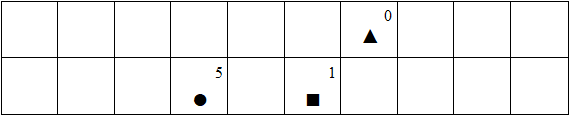
\includegraphics[width=0.75\textwidth]{problem-beispiel}
 \caption[Problem-Beispiel]{Beispiel für ein Problem-Szenario, drei Fahrzeuge und deren Geschwindigkeiten}
 \label{figure:problem-beispiel}
\end{figure}

In \ref{figure:problem-beispiel} wird dem Fahrzeug \textbf{CIRCLE} nach dem Multi-Lane-Modell aus \cite{multi-lane} das Ausscheren vorgegeben, denn die linke Spur bietet mehr Platz als die rechte. 
Das Fahrzeug $\blacktriangle$ ist drei Felder vor \textbf{CIRCLE}.
Ein Abbremsen von \textbf{CIRCLE} auf $v=2$ würde veranlasst.
Dass $\blacktriangle$ gleichzeitig um $1$ beschleunigen könnte, spielt keine Rolle. \\
Nach dem "Social-Force-Modell" würde dem Fahrzeug \textbf{CIRCLE} wahrscheinlich eine höhere Kraft der entsprechenden Zelle und somit Wahrscheinlichkeit für das Ausscheren berechnet werden.
Dies muss aber nicht zur Entscheidung in Richtung Spurwechsel führen.
$\blacksquare$ kann im aktuellen Zeitschritt max. auf $v=2$ beschleunigen, $\blacktriangle$ max. auf $v=1$.
Da das Fahrzeug \textbf{CIRCLE} seine Geschwindigkeit aber nur durch die Zufallsgröße "Trödeln" um $1$ reduzieren kann, würde es beim Setzen/Fahren auf das gleiche Grid-Feld oder gar davor gesetzt werden.